
\de{ĐỀ THI GIỮA HỌC KỲ II NĂM HỌC 2022-2023}{THPT Tân Bình}


\begin{center}
	\textbf{PHẦN 1 - TRẮC NGHIỆM}
\end{center}


\Opensolutionfile{ans}[ans/ans]



% Câu 1 - Trác nghiệm
\begin{ex}%[0T7Y2-1]%[Dự án đề kiểm tra GKII NH22-23 - Quan Ón]%[Tân Bình]
	Bất phương trình $x^2 - 2x - 3 > 0$ nhận giá trị nào dưới đây là một nghiệm?
	\choice
	{\True $-2$}
	{$3$}
	{$0$}
	{$-1$}
	\loigiai{
		Thay $x = -2$ vào bất phương trình, ta được $(-2)^2 - 2\cdot (-2) - 3 > 0 \Leftrightarrow 5 > 0$ (luôn đúng).\\
		Do đó $x = -2$ là một nghiệm của bất phương trình đã cho.
	}
\end{ex}

% Câu 2 - Trác nghiệm
\begin{ex}%[0T7B3-2]%[Dự án đề kiểm tra GKII NH22-23 - Quan Ón]%[Tân Bình]
	Phương trình nào dưới đây nhận $x = 0$ là nghiệm?
	\choice
	{$\sqrt{x + 1} = -1$}
	{$\sqrt{x-9} = 3$}
	{\True $\sqrt{x} = -x$}
	{$\sqrt{4-x} = x - 2$}
	\loigiai{
		Xét phương trình $\sqrt{x} = -x$.\\
		Điều kiện $x \geq 0$.\\
		Thay $x = 0$ vào phương trình trên, ta được $\sqrt{0} = -0 \Leftrightarrow 0 = 0$ (luôn đúng).\\
		Vậy $x = 0$ là nghiệm của phương trình $\sqrt{x} = -x$.
	}
\end{ex}

% Câu 3 - Trác nghiệm
\begin{ex}%[0T9Y3-1]%[Dự án đề kiểm tra GKII NH22-23 - Quan Ón]%[Tân Bình]
	Trong mặt phẳng $Oxy$, phương trình $x^2 + y^2 - 2ax - 2by + c = 0$ là phương trình đường tròn khi và chỉ khi
	\choice
	{$a^2 + b^2 - c \geq 0$}
	{$a^2 + b^2 - c^2 >0$}
	{$a^2 + b^2 - c^2 \geq 0$}
	{\True $a^2 + b^2 - c > 0$}
	\loigiai{
		Trong mặt phẳng $Oxy$, phương trình $x^2 + y^2 - 2ax - 2by + c = 0$ là phương trình đường tròn khi và chỉ khi $a^2 + b^2 - c > 0$.
	}
\end{ex}

% Câu 4 - Trác nghiệm
\begin{ex}%[0T7B1-1] %[Dự án đề kiểm tra GKII NH22-23 - Quan Ón]%[Tân Bình]
	Tam thức bậc hai $f(x) = 4 - x^2$ dương tại giá trị nào dưới đây?
	\choice
	{$x_2 = 3$}
	{\True $x_1 = -1$}
	{$x_3 = -5$}
	{$x_0 = 2$}
	\loigiai{
		Thay $x_1 = -1$ vào tam thức bậc hai, ta được $f(-1) = 4 - (-1)^2 = 4 - 1 = 3 > 0$.\\
		Vậy tam thức bậc hai $f(x) = 4 - x^2$ dương tại giá trị $x_1 = -1$.
	}
\end{ex}

% Câu 5 - Trác nghiệm
\begin{ex}%[0T9B2-6]%[Dự án đề kiểm tra GKII NH22-23 - Quan Ón]%[Tân Bình]
	Trong mặt phẳng $Oxy$, cho đường thẳng $d\colon \heva{&x = 1 + t\\&y = 3 - 2t}$. Điểm nào dưới đây thuộc $d$?
	\choice
	{$P(1;-2)$}
	{$Q(-2;1)$}
	{\True $M(1;3)$}
	{$N(3;1)$}
	\loigiai{
		Dựa vào phương trình, ta thấy đường thẳng $d$ đi qua điểm $M(1;3)$.
	}
\end{ex}



% Câu 6 - Trác nghiệm
\begin{ex}%[0T7B1-1] %[Dự án đề kiểm tra GKII NH22-23 - Quan Ón]%[Tân Bình]
	Biết tam thức bậc hai $f(x) = ax^2 + bx + c$ có $a > 0$, $\Delta = b^2 - 4ac = 0$. Khẳng định nào dưới đây đúng?
	\choice
	{$f(x) < 0$, $\forall x \in \mathbb{R}$}
	{$f(x) > 0$, $\forall x \in \mathbb{R}$}
	{$f(x) \leq 0$, $\forall x \in \mathbb{R}$}
	{\True $f(x) \geq 0$, $\forall x \in \mathbb{R}$}
	\loigiai{
		Vì tam thức bậc hai $f(x)$ có $\heva{&a > 0\\&\Delta = 0}$ nên $f(x) \geq 0$, $\forall x \in \mathbb{R}$.
	}
\end{ex}

% Câu 7 - Trác nghiệm
\begin{ex}%[0T9Y3-1] %[Dự án đề kiểm tra GKII NH22-23 - Quan Ón]%[Tân Bình]
	Trong mặt phẳng $Oxy$, cho đường tròn $(C)\colon (x + 2)^2 + (y - 1)^2 = 25$. Tâm của $(C)$ có tọa độ là
	\choice
	{\True $(-2;1)$}
	{$(-2;-1)$}
	{$(2;-1)$}
	{$(2;1)$}
	\loigiai{
		Tâm của đường tròn $(C)$ có tọa độ là $(-2;1)$.
	}
\end{ex}

% Câu 8 - Trác nghiệm
\begin{ex}%[0T9B1-2]%[Dự án đề kiểm tra GKII NH22-23 - Quan Ón]%[Tân Bình]
	Trong mặt phẳng $Oxy$, cho $\overrightarrow{a} = 2\overrightarrow{i} - 3\overrightarrow{j}$. Tọa độ của véc-tơ $\overrightarrow{a}$ là
	\choice
	{$(-3;2)$}
	{$(3;-2)$}
	{\True $(2;-3)$}
	{$(-2;3)$}
	\loigiai{
		Vì $\overrightarrow{a} = 2\overrightarrow{i} - 3\overrightarrow{j}$ nên  $\overrightarrow{a} = (2;-3)$.
	}
\end{ex}

% Câu 9 - Trác nghiệm
\begin{ex}%[0T7B2-1]%[Dự án đề kiểm tra GKII NH22-23 - Quan Ón]%[Tân Bình]
	Biết tam thức bậc hai $f(x)$ có bảng xét dấu như trong hình vẽ. Tập nghiệm của bất phương trình $f(x) \geq 0$ là
	\begin{center}
		
\begin{tikzpicture}[scale=1, font=\footnotesize, line join=round, line cap=round, >=stealth]
			\tkzTabInit[nocadre=false,lgt=1.2,espcl=2.5,deltacl=0.6]
			{$x$ /0.6,$f(x)$/0.8}
			{$-\infty$,$0$, $2$, $+\infty$}
			\tkzTabLine{,-,0,+,0,-,}
		\end{tikzpicture}
	\end{center}
	\choice
	{$(-\infty; 0) \cup (2;+\infty)$}
	{\True $[0;2]$}
	{$(0;2)$}
	{$(-\infty; 0]\cup [2;+\infty)$}
	\loigiai{
		Dựa vào bảng xét dấu, ta có $f(x) \geq 0 \Leftrightarrow x \in [0;2]$.\\
		Vậy tập nghiệm của bất phương trình $f(x) \geq 0$ là $[0;2]$.
	}
\end{ex}

% Câu 10 - Trác nghiệm
\begin{ex}%[0T7Y2-1]%[Dự án đề kiểm tra GKII NH22-23 - Quan Ón]%[Tân Bình]
	Bất phương trình nào dưới đây là bất phương trình bậc hai một ẩn $x$?
	\choice
	{$1 - x \leq 0$}
	{\True $9 - x^2 > 0$}
	{$x(x^2 - 3x + 2) > 0$}
	{$2x^2 - 3x^3 + 1 \leq 0$}
	\loigiai{
		Bất phương trình bậc hai một ẩn $x$ là $9 - x^2 > 0$.
	}
\end{ex}



% Câu 11 - Trác nghiệm
\begin{ex}%[0T9Y1-3] %[Dự án đề kiểm tra GKII NH22-23 - Quan Ón]%[Tân Bình]
	Trong mặt phẳng $Oxy$, cho hai điểm bất kì $A(x_A; y_A)$ và $B(x_B;y_B)$. Tọa độ của véc-tơ $\overrightarrow{AB}$ là
	\choice
	{$(x_B + x_A; y_B + y_A)$}
	{$(x_Ax_B; y_Ay_B)$}
	{\True $(x_B - x_A; y_B - y_A)$}
	{$(x_A - x_B; y_A - y_B)$}
	\loigiai{
		Vì $A(x_A; y_A)$ và $B(x_B;y_B)$ nên $\overrightarrow{AB} = (x_B - x_A; y_B - y_A)$.
	}
\end{ex}

% Câu 12 - Trác nghiệm
\begin{ex}%[0T7B2-1]%[Dự án đề kiểm tra GKII NH22-23 - Quan Ón]%[Tân Bình]
	\immini{
	Cho hàm số bậc hai $y = f(x)$ có đồ thị như trong hình vẽ. Khẳng định nào dưới đây đúng?
	\choice
	{\True $f(x) > 0$, $\forall x \in (-\infty;-1)\cup (2;+\infty)$}
	{$f(x) >0$, $\forall x \in (-\infty;-1]\cup [2;+\infty)$}
	{$f(x) > 0$, $\forall x \in (-1;2)$}
	{$f(x) > 0$, $\forall x \in [-1;2]$}
}{
    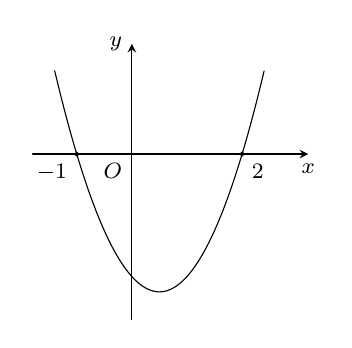
\begin{tikzpicture}[scale=0.7, font=\footnotesize, line join=round, line cap=round, >=stealth]
    	\def\xt{-1.8} \def\xp{3.2} \def\yt{2} \def\yd{-3}
    	\draw[->] (\xt,0)--(\xp,0) node [below]{$x$};
    	\draw[->] (0,\yd)--(0,\yt) node [left]{$y$};
    	\node at (0,0) [below left]{$O$} circle (1pt);
    	\draw (-1,0) node[below left]{$-1$} circle (1pt);
    	\draw (2,0) node[below right]{$2$} circle (1pt);
    	\clip (\xt,\yd) rectangle (\xp,\yt);
    	\draw [smooth, domain=-1.4:2.4, samples=100] %
    	plot (\x, {1.1111*(\x)^2 - 1.1111*(\x) - 2.2222});
    \end{tikzpicture}
}
	\loigiai{
		Dựa vào đồ thị, ta có $f(x) > 0$, $\forall x \in (-\infty;-1)\cup (2;+\infty)$.
	}
\end{ex}

% Câu 13 - Trác nghiệm
\begin{ex}%[0T7Y1-1]%[Dự án đề kiểm tra GKII NH22-23 - Quan Ón]%[Tân Bình]
	Đa thức nào dưới đây là một tam thức bậc hai?
	\choice
	{$g(x) = x^4 - x^2 + 3$}
	{$f(x) = 2x - 1$}
	{$k(x) = 2x^3 + x^2 + 1$}
	{\True $h(x) = x^2 - 3x$}
	\loigiai{
		Đa thức $h(x) = x^2 - 3x$ là một tam thức bậc hai.
	}
\end{ex}

% Câu 14 - Trác nghiệm
\begin{ex}%[0T9Y1-2]%[Dự án đề kiểm tra GKII NH22-23 - Quan Ón]%[Tân Bình]
	Trong mặt phẳng $Oxy$, cho hai véc-tơ $\overrightarrow{u} = (3;-2)$ và $\overrightarrow{v} = (-2;1)$. Tọa độ của véc-tơ $\overrightarrow{u} + \overrightarrow{v}$ là 
	\choice
	{$(-1;1)$}
	{$(3;-5)$}
	{\True $(1;-1)$}
	{$(5;-3)$}
	\loigiai{
		Ta có $\overrightarrow{u} + \overrightarrow{v} = \left( 3 + (-2);(-2) + 1 \right) = (1;-1)$.
	}
\end{ex}


%Câu 15...........................
\begin{ex}%[0T9Y2-1]%[Dự án đề kiểm tra GKII NH22-23 - Nguyễn Văn Sơn]%[Tân Bình]
	Trong mặt phẳng $Oxy$, cho đường thẳng $d\colon 2x-3y+1=0$. Vectơ nào dưới đây là một vectơ pháp tuyến của $d$?
	\choice
	{$\vec a=\left(2;3\right)$}
	{$\vec b=\left(3;2\right)$}
	{ $\vec v=\left(-3;2\right)$}
	{\True $\vec w=\left(2;-3\right)$}
	\loigiai{
		Do đường thẳng $d$ có phương trình tổng quát là $2x-3y+1=0$ nên ta có vectơ pháp tuyến của đường thẳng là $\vec w=\left(2;-3\right)$.
	}
\end{ex}
%%==========Câu 16
\begin{ex}%[0T9Y2-5]%[Dự án đề kiểm tra GKII NH22-23 - Nguyễn Văn Sơn]%[Tân Bình]
	Trong mặt phẳng $Oxy$ cho đường thẳng $d\colon Ax+By+C=0$ với $\left(A^2+B^2\neq 0\right)$ và điểm $M\left(x_0;y_0\right)$ tuỳ ý. Khoảng cách từ $M$ đến $d$ bằng
	\choice
	{$\dfrac{Ax_0+By_0+C}{{A^2+B^2}}$}
	{$\dfrac{\left|Ax_0+By_0+C\right|}{A^2+B^2}$}
	{$\dfrac{Ax_0+By_0+C}{\sqrt{A^2+B^2}}$}
	{\True $ \dfrac{\left|Ax_0+By_0+C\right|}{\sqrt {A^2+B^2}}$}
	\loigiai{
		Theo định nghĩa sách giáo khoa ta có công thức tính khoảng cách từ điểm $M\left(x_0;y_0\right)$ đến đường thẳng $d:Ax+By+C=0$ là  $\mathrm{d}(M,d)=\dfrac{\left|Ax_0+By_0+C\right|}{\sqrt{A^2+B^2}}$.
	}
\end{ex}
%%==========Câu 17
\begin{ex}%[0T9B2-2]%[Dự án đề kiểm tra GKII NH22-23 - Nguyễn Văn Sơn]%[Tân Bình]
	Phương trình tổng quát của đường thẳng đi qua hai điểm $A\left(1;2\right)$ và $B\left(-1;-1\right)$ là
	\choice
	{\True$2x+3y-8=0$}
	{$3x-2y+1=0$}
	{$3x-2y-1=0$}
	{ $2x+3y+8=0$}
	\loigiai{
		Ta có $\overrightarrow{AB}=\left(-2;-3\right)$ nên $\overrightarrow{n}=\left(2;3\right)$ là một véc-tơ pháp tuyến của đường thẳng $AB$.\\
		Khi đó phương trình tổng quát của đường thẳng $AB$ là\\
		$$AB: 2\left(x-1\right)+3\left(y-2\right)=0\Leftrightarrow 2x+3y-8=0$$.
	}
\end{ex}
%%==========Câu 18
\begin{ex}%[0T9B3-2]%[Dự án đề kiểm tra GKII NH22-23 - Nguyễn Văn Sơn]%[Tân Bình]
	Trong mặt phẳng $Oxy$, đường tròn tâm $I(3;-4)$ và đi qua điểm $O$ có phương trình là
	\choice
	{\True $(x-3)^2+(y+4)^2=25$}
	{$(x-3)^2+(y+4)^2=5$}
	{$(x+3)^2+(y-4)^2=25$}
	{$(x+3)^2+(y-4)^2=5$}
	\loigiai{
		Đường tròn $(C)$ có tâm $I(3;-4)$ và bán kính $R$ có phương trình dạng
		\begin{center}
		$(x-3)^2+(y+4)^2=R^2$.
		\end{center}
		$O(0;0)\in (C)$ nên bán kính của đường tròn là\\
		$R=OM=\sqrt{(3-0)^2+(-4-0)^2}$ $=\sqrt{25}=5$. \\
		Vậy phương trình đường tròn là $(x-3)^2+(y+4)^2=25$.
	}
	
\end{ex}
%%==========Câu 19
\begin{ex}%[0T7B2-1]%[Dự án đề kiểm tra GKII NH22-23 - Nguyễn Văn Sơn]%[Tân Bình]
	Bất phương trình nào dưới đây có tập nghiệm là $\mathbb{R}$?
	\choice
	{\True$x^2+x+1\geq 0$}
	{$x^2-6x+9>0$}
	{$3x-4>0$}
	{$4-x^2\leq 0$}
	\loigiai{
		Xét $f\left(x\right)=x^2+x+1=0$ vô nghiệm và có $a=1>0$ nên $f\left(x\right)>0\ \forall x\in\mathbb{R}$.\\
		Do đó bất phương trình $x^2+x+1\geq 0$ có tập nghiệm là $\mathbb{R}$.
	}
\end{ex}
%%==========Câu 20
\begin{ex}%[0T7B3-2]%[Dự án đề kiểm tra GKII NH22-23 - Nguyễn Văn Sơn]%[Tân Bình]
	Phép biến đổi nào dưới đây đúng?
	\choice
	{\True$\sqrt{x^2}=2\Rightarrow x^2=4$}
	{$x^2=4\Rightarrow x=2$}
	{$\sqrt{x^2+9}=2x-3\Rightarrow x^2+9=2x-3$}
	{$\sqrt{x^2+9}=2x-3\Rightarrow x+3=2x-3$}
	\loigiai{
		Ta có phép biến đổi $\sqrt{x^2}=2\Rightarrow x^2=4$ là đúng.
	}
\end{ex}
%%==========Câu 21
\begin{ex}%[0T9B1-2]%[Dự án đề kiểm tra GKII NH22-23 - Nguyễn Văn Sơn]%[Tân Bình]
	Trong mặt phẳng $Oxy$, xét các vec-tơ $\overrightarrow{u}=(3;m+1), \overrightarrow{v}=(n+1;-3)$. Khi $\overrightarrow{u}=\overrightarrow{v}$, giá trị $m+n$ bằng
	\choice
	{$2$}
	{\True $-2$}
	{$-6$}
	{$0$}
	\loigiai
	{
		Ta có $\overrightarrow {u}=\overrightarrow{v}$ 
		$\Leftrightarrow$
		$\heva{&3=n+1\\&m+1=-3}$
		$\Leftrightarrow$
		$\heva{&n=2\\&m=-4.}$\\
		Suy ra $m+n=-2$.
	}
\end{ex}
%%==========Câu 22
\begin{ex}%[0T7B1-1]%[Dự án đề kiểm tra GKII NH22-23 - Nguyễn Văn Sơn]%[Tân Bình]
	Tam thức bậc hai nào có bảng xét dấu như hình vẽ?
	\begin{center}
		
\begin{tikzpicture}[scale=1]
			\tkzTabInit[lgt=1,espcl=1.5]
			{$x$  /0.6,$f(x)$  /0.6}
			{$-\infty$,$ -3 $, $ 2 $,$+\infty$}
			\tkzTabLine{,+,0,-,0,+,}
		\end{tikzpicture}
	\end{center}
	\choice
	{$f(x)=-x^2+x+6$}
	{$f(x)=-2x^2-2x+12$}
	{\True $f(x)=2x^2+2x-12$}
	{$f(x)=x^2-x-6$}
	\loigiai
	{ 
		Dựa vào bảng xét dấu ta có tam thức $f(x)=0$ có hai nghiệm $x_1=-3; x_2=2$ và hệ số $a>0$. Chỉ có tam thức $f(x)=2x^2+2x-12$ thoả mãn.
	}
\end{ex}
%%==========Câu 23
\begin{ex}%[0T9K1-3]%[Dự án đề kiểm tra GKII NH22-23 - Nguyễn Văn Sơn]%[Tân Bình]
	Trong mặt phẳng $Oxy$, cho $A(-1;-2)$. Một chất điểm $M$ từ vị trí điểm $A$ chuyển động thẳng đều với vectơ vận tốc $\overrightarrow{v}=(-3;4)$. Khoảng cách ngắn nhất giữa chất điểm $M$ và $O$ bằng
	\choice
	{$\sqrt{5}$}
	{$5$}
	{\True $2$}
	{$\dfrac{2}{5}$}
	\loigiai
	{ Vì chất điểm $M(x;y)$ chuyển động thẳng đều với vận tốc $\overrightarrow{v}=(-3;4)$ nên ta có $\overrightarrow{AM}=k\overrightarrow{v}$.\\ Suy ra 
		$\heva{&x+1=-3k\\&y+2=4k} \Leftrightarrow \heva {&x=-1-3k\\&y=4k-2.}$\\
		Suy ra $OM=\sqrt{(-1-3k)^2+(4k-2)^2}=\sqrt{25k^2-10k+5}=\sqrt{(5k-1)^2+4}\ge \sqrt{4}=2$.
		Suy ra $OM$ nhỏ nhất là $2$.
	}
\end{ex}
%%==========Câu 24
\begin{ex}%[0T9K1-3]%[Dự án đề kiểm tra GKII NH22-23 - Nguyễn Văn Sơn]%[Tân Bình]
	Trong mặt phẳng $Oxy$, cho hai đường thẳng $d_1\colon\heva{&x=t\\&y=-1+t},d_2\colon 3x-y-5=0$ và điểm $M(2;2)$. Gọi $A$, $B$ lần lượt thuộc $d_1$ và $d_2$ sao cho $M$ là trung điểm $AB$. Giá trị $OA+OB$ bằng
	\choice
	{$4\sqrt{2}$}
	{$26$}
	{$8$}
	{\True$6$}
	\loigiai
	{
		Gọi điểm $A(t;-1+t)\in d_1$. Giả sử $B(x;y)\in d_2$. Vì $M(2;2)$ là trung điểm $AB$ nên ta có $\heva{&\dfrac{t+x}{2}=2\\&\dfrac{-1+t+y}{2}=2}$ $\Leftrightarrow \heva{&t+x=4\\&t+y=5} \Leftrightarrow \heva{&x=4-t\\&y=5-t}.$\\
		Thay vào đường thẳng $d_2$ ta có: $3(4-t)-(5-t)-5=0$.\\ Suy ra $t=1$ nên $A(1;0)$, $B(3;4)$ nên $OA+OB=\sqrt{1^2+0^2}+\sqrt{3^2+4^2}=1+5=6.$ 
	}
\end{ex}
%%==========Câu 25
\begin{ex}%[0T3T2-5]%[Dự án đề kiểm tra GKII NH22-23 - Nguyễn Văn Sơn]%[Tân Bình]
		Một công ty cầu đường muốn thiết kế một hầm đường bộ có dạng parabol, khoảng cách từ mặt đường đến đỉnh hầm bằng $h$, chiều rộng mặt đường $14$ mét được chia đều thành $4$ làn xe, (giả sử vạch kẻ đường có kích thước không đáng kể). Tìm giá trị nhỏ nhất của $h$ để một chiếc xe chở hàng có chiều rộng $2{,}5$ mét và chiều cao $5$ mét, khi đi đúng làn đường số $3$ (trên hình vẽ) luôn có thể qua hầm an toàn (tức là khoảng cách từ mặt trên cùng của thùng xe đến mặt hầm không nhỏ hơn $1$ mét)?
	
			\begin{center}
			 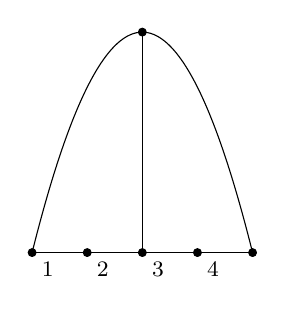
\begin{tikzpicture}[scale=0.7, font=\footnotesize, line join=round, line cap=round, >=stealth]
				\def\xt{-2} \def\xp{2} \def\yt{4} \def\yd{0}
				\draw (\xt,0)--(\xp,0); %node [below]{$x$};
				\draw (0,\yd)--(0,\yt); %node [left]{$y$};
%				\node at (0,0) [below left]{$O$} circle (1pt);
				\filldraw (-2,0) node[below right]{$1$} circle (2pt);
				\filldraw (-1,0) node[below right]{$2$} circle (2pt);
				\filldraw (0,0) node[below right]{$3$} circle (2pt);
				\filldraw (1,0) node[below right]{$4$} circle (2pt);
				\filldraw[black] (2,0) circle (2pt);
				\filldraw (0,4) circle (2pt);
				\clip (\xt,\yd) rectangle (\xp,\yt);
				\draw [smooth, domain=-3:3, samples=100] %
				plot (\x, {-1.0*(\x)^2+4});
			\end{tikzpicture}
		\end{center}
	\choice
	{$7$ mét}
	{\True $8$ mét}
	{$7{,}5$ mét}
	{$6{,}7$ mét}
	\loigiai{
			Chiều rộng của một làn xe là $14:4=3{,5}$ m.\\
			Xét xe tải đi sát phía bên ngoài bên phải làn thứ $3$ (minh họa như hình bên dưới), vị trí này xe tải sẽ gần mặt hầm nhất.\\
			Càng về phía bên phải, chiều cao hầm càng giảm, để xe qua an toàn thì khoảng cách từ mặt đất đến mặt hầm theo phương vuông góc với mặt đất và đi qua giao giữa làn số $3$ và làn số $4$ phải lớn hơn hoặc bằng $5+1=6$ (m).\\
			Gắn hệ trục tọa độ như hình vẽ.\\
			Parabol đối xứng qua trục $Oy$ có phương trình: $y=a^2+c (c\ne 0) (P)$.\\
			$(P)$ đi qua $(3{,}5;6)$ và $(7;0)$ nên ta có $\heva{&6=a\cdot \left(3{,5}\right)^2 +c\\& 0=a\cdot \left(7\right)^2+c}$ $\Rightarrow$ $\heva{& a=-\dfrac{8}{49}\\&c=8.}$\\
			Suy ra chiều cao hầm $h=y(0)=c=8$ mét.\\
			\begin{center}
				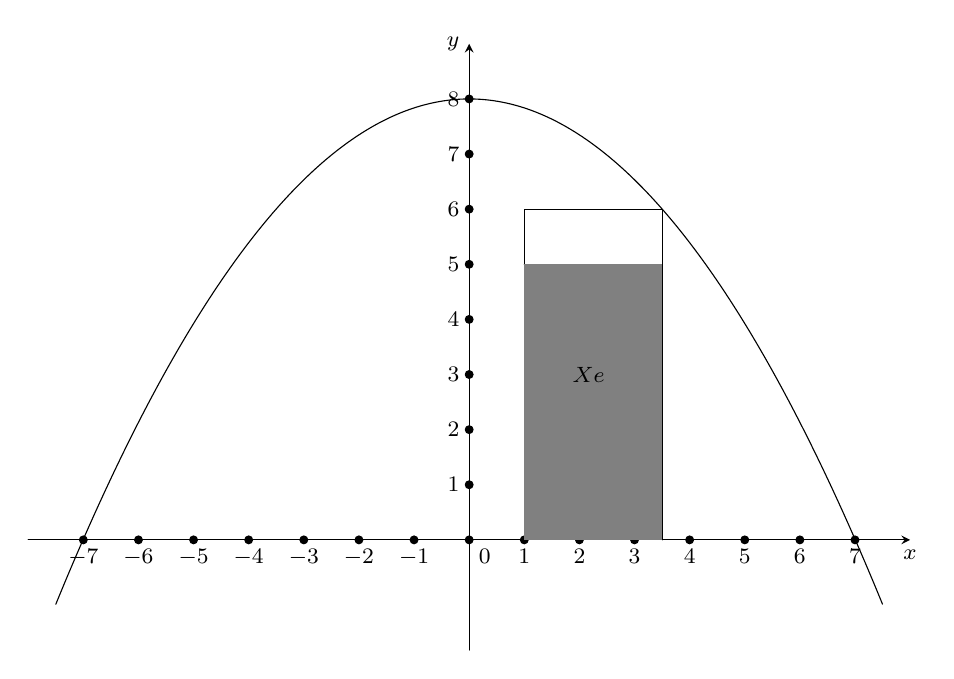
\begin{tikzpicture}[scale=0.7, font=\footnotesize, line join=round, line cap=round, >=stealth]
				\def\xt{-8} \def\xp{8} \def\yt{9} \def\yd{-2}
				\draw [->](\xt,0)--(\xp,0); %node [below]{$x$};
				\draw [->](0,\yd)--(0,\yt); %node [left]{$y$};
				\foreach \x/\y in {-7/0,-6/0,-5/0,-4/0,-3/0,-2/0,-1/0,1/0,2/0,3/0,4/0,5/0,6/0,7/0}{\filldraw (\x,\y) node[below]{$\x$} circle (2pt);}
				\foreach \x/\y in {0/1,0/2,0/3,0/4,0/5,0/6,0/8,0/7}{\filldraw (\x,\y) node[left]{$\y$} circle (2pt);}
				\filldraw (0,0) node[below right]{$0$} circle (2pt);
				\filldraw (0,9) node[left]{$y$};
				\filldraw (8,0) node[below]{$x$};
				\draw (1,0)--(1,6) -- (3.5,6)-- (3.5,0);
				\draw (1,5)--(3.5,5);
				\fill[gray] (1,0) rectangle(3.5,5);
				\filldraw (1.7,3) node[right]{$Xe$};
%				\filldraw (-1,0) node[below right]{$2$} circle (2pt);
%				\filldraw (0,0) node[below right]{$3$} circle (2pt);
%				\filldraw (1,0) node[below right]{$4$} circle (2pt);
%				\filldraw[black] (2,0) circle (2pt);
%				\filldraw (0,4) circle (2pt);
%				\clip (\xt,\yd) rectangle (\xp,\yt);
				\draw [smooth, domain=-7.5:7.5, samples=100] %
				plot (\x, {-0.163*(\x)^2+8});
			\end{tikzpicture}
			\end{center}
			}
\end{ex}

%%==========Câu 26
\begin{ex}%[0T9K1-3]%[Dự án đề kiểm tra GKII NH22-23 - Nguyễn Văn Sơn]%[Tân Bình]
	Trong mặt phẳng $Oxy$, cho hai điểm $A(1;2)$ và $B(0;1)$. Gọi $C$ là điểm thuộc trục $Ox$ sao cho tam giác $ABC$ vuông tại $B$. Tâm đường tròn ngoại tiếp tam giác $ABC$ có tọa độ là
	\choice
	{$\left(\dfrac{1}{2};\dfrac{3}{2}\right)$}
	{$\True \left(1;1\right)$}
	{$\left(\dfrac{1}{2};\dfrac{1}{2}\right)$}
	{$\left(\dfrac{2}{3};\dfrac{4}{3}\right)$}
	\loigiai{
	$C$ thuộc trục $Ox$ nên $C\left(x;0\right)$	.\\
	$\overrightarrow{AB}=(-1;-1)$, $\overrightarrow{BC}=(x;-1)$.\\
	Tam giác $ABC$ vuông tại $B$ nên $AB$ vuông góc $BC$ suy ra $\overrightarrow{AB}\cdot\overrightarrow{BC}=0$.\\
	Suy ra $(-1)\cdot x + (-1)\cdot (-1)=0 \Rightarrow x=1\Rightarrow C(1;0)$.\\
	Tam giác $ABC$ vuông tại $B$ nên có tâm đường tròn ngoại tiếp là trung điểm $AC$ và có tọa độ là $(1;1)$.
	}
\end{ex}
%%==========Câu 27
\begin{ex}%[0T9K2-2]%[Dự án đề kiểm tra GKII NH22-23 - Nguyễn Văn Sơn]%[Tân Bình]
	Trong mặt phẳng $Oxy$, cho điểm $M\left(-2;2\right)$ thuộc đường thẳng $d:x+my+n=0$. Biết đường thẳng $d$ cắt $Ox,Oy$ lần lượt tại $A$ và $B$ sao cho tam giác $OAB$ cân. Giá trị $m+n$ bằng
\choice
{\True $3$}
{$2$}
{$0$}
{$-5$}
\loigiai{
	$A,B$ lần lượt thuộc trục $Ox,Oy$ nên tọa độ có dạng $A(a;0)$, $B(0,b)$.\\
	Phương trình đường thẳng $d$ đi qua $A$,$B$ là phương trình đoạn chắn có dạng: $\dfrac{x}{a} + \dfrac{y}{b}=1$.\\
	$d$ đi qua $M(-2;2)$ nên ta có:  $\dfrac{-2}{a} + \dfrac{2}{b}=1$. (*)\\
	Tam giác $OAB$ cân nên $OA=OB$, do đó ta có $2$ trường hợp sau:\\
	TH1: $a=b$ thế vào phương trình (*) ta có $0=1$ (vô lý).\\
	TH2: $a=-b$ thế vào phương trình (*) ta có $\dfrac{4}{b}=1$ suy ra $b=4 \Rightarrow a=-4$.\\
	Suy ra phương trình $d$ là $\dfrac{x}{-4}+\dfrac{y}{4}=1 \Leftrightarrow x-y+4=0$.\\
	Suy ra $m=-1$ và $n=4$, do đó $m+n = 3$.
}
\end{ex}
%%==========Câu 28
\begin{ex}%[0T7K1-1]%[Dự án đề kiểm tra GKII NH22-23 - Nguyễn Văn Sơn]%[Tân Bình]
	Xét hàm số $f(x)=\sqrt{x^2-2\left(m+1\right)x+7m+15}$ ($m$ là tham số). Có bao nhiêu giá trị $m$ nguyên để hàm số $f(x)$ có tập xác định là $\mathbb{R}$?
\choice
{$8$}
{$7$}
{$9$}
{$10$}
\loigiai{
	Hàm số $f(x)$ có tập xác định là $\mathbb{R}$ khi $x^2-2\left(m+1\right)x+7m+15 \ge 0, \forall x\in\mathbb{R} $.\\
	$\Leftrightarrow \heva{&a>0\\&\Delta'\le 0}$ $\Leftrightarrow\heva{&1>0\\&\left(m+1\right)^2-\left(7m+15\right)\le 0}$ 
	\\$\Leftrightarrow m^2-5m-14 \le 0\Leftrightarrow -2\le m \le 7$.\\
	Suy ra $m\in \{-2;-3;-1;0;1;2;3;4;5;6;7\}$. \\Nên có $10$ giá trị $m$ nguyên thỏa yêu cầu bài toán.
	
}
\end{ex}



\Closesolutionfile{ans}


\begin{center}
	\textbf{PHẦN 2 - TỰ LUẬN}
\end{center}


\begin{bt}%[0T7B2-1]%[Dự án đề kiểm tra NH22-23 - Huỳnh Quy]%[THPT Tân Bình]
Lập bảng xét dấu của $f(x)=-2x^2+5x-2$, suy ra tập nghiệm của bất phương trình $f(x)>0$.	
\loigiai{
	Hệ số $a=-2<0$.\\
	$\Delta=5^2-4\cdot(-2)\cdot (-2)=9>0$.\\
	$f(x)=0\Leftrightarrow \hoac{&x=2\\&x=\dfrac{1}{2}.}$\\
	Bảng xét dấu:
	\begin{center}
		
\begin{tikzpicture}[scale=1]
			\tkzTabInit[lgt=1,espcl=1.5]
			{$x$ /0.6, $f(x)$ /0.6}
			{$-\infty$, $\tfrac{1}{2}$, $ 2 $,$+\infty$}
			\tkzTabLine{,-,0,+,0,-,}
		\end{tikzpicture}
	\end{center}
	Dựa vào bảng xét dấu ta có tập nghiệm của bất phương trình $f(x)>0$ là $S=\left(\dfrac{1}{2};2\right)$. 
}
\end{bt}

\begin{bt}%[0T7B3-2]%[Dự án đề kiểm tra NH22-23 - Huỳnh Quy]%[THPT Tân Bình]
	Giải phương trình $3\sqrt{x^2-x-1}=2x-1$.
	\loigiai{
		Bình phương hai vế phương trình đã cho ta được
		\begin{eqnarray*}
			&&9(x^2-x-1)=(2x-1)^2\\
			&\Rightarrow&9(x^2-x-1)=4x^2-4x+1\\
			&\Rightarrow&5x^2-5x-10=0\\
			&\Rightarrow&\hoac{&x=2\\&x=-1.}
		\end{eqnarray*}
	Thử lại, ta thay các giá trị $x=2$, $x=-1$ vào phương trình ban đầu thì chỉ có giá trị $x=2$ thỏa mãn.\\
	Vậy phương trình có nghiệm $x=2$.
	}
\end{bt}

\begin{bt}%[0T9K2-2]%[Dự án đề kiểm tra NH22-23 - Huỳnh Quy]%[THPT Tân Bình]
	Trong mặt phẳng $Oxy$, cho tam giác $ABC$ có $A(-2;0)$, $B(-1;4)$ và $C(4;3)$. Viết phương trình đường thẳng đi qua $C$, cắt cạnh $AB$ tại điểm $D$ sao cho hai tam giác $BCD$ và $ACD$ có diện tích bằng nhau.
	\loigiai{
		Ta có $S_{\triangle ACD}=\dfrac{1}{2}AD\cdot\mathrm{d}(C,AB)$; $S_{\triangle BCD}=\dfrac{1}{2}BD\cdot\mathrm{d}(C,BD)$.\\
		Ta có $S_{\triangle ACD}=S_{\triangle BCD}\Rightarrow AD=BD$.\\
		Do đó $D$ là trung điểm của $AB$.\\
		Gọi $D(x_D;y_D)$. Ta có $\heva{&x_D=\dfrac{x_A+x_B}{2}=\dfrac{(-2)+(-1)}{2}=-\dfrac{3}{2}\\&y_D=\dfrac{y_A+y_B}{2}=\dfrac{0+4}{2}=2}\Rightarrow D\left(-\dfrac{3}{2};2\right)$.\\
		Phương trình đường thẳng $d$ đi qua hai điểm $C(4;3)$ và $D\left(-\dfrac{3}{2};2\right)$ là
		\begin{eqnarray*}
			&&\dfrac{x-x_C}{x_D-x_C}=\dfrac{y-y_C}{y_D-y_C}\\
			&\Leftrightarrow&\dfrac{x-4}{-\dfrac{3}{2}-4}=\dfrac{y-3}{2-3}\\
			&\Leftrightarrow&-(x-4)=-\dfrac{11}{2}(y-3)\\
			&\Leftrightarrow&\boxed{2x-11y+25=0}.
		\end{eqnarray*}
	}
\end{bt}

\begin{bt}%[0T7G1-1]%[Dự án đề kiểm tra NH22-23 - Huỳnh Quy]%[THPT Tân Bình]
	Chứng minh $3x^2+2y^2-2xy-4x-2y+3\geq 0$, $\forall x,y\in\mathbb{R}$.
	\loigiai{
		Xét biểu thức 
		\begin{eqnarray*}
			f(x;y)&=&3x^2+2y^2-2xy-4x-2y+3\\
			&=&3x^2-(2y+4)x+2y^2-2y+3.
		\end{eqnarray*}
	Ta xem $f(x;y)$ là một tam thức bậc hai theo biến $x$, xem $y$ là tham số.\\
	Tam thức này có biệt thức 
	\begin{eqnarray*}
		\Delta_x&=&[-(2y+4)]^2-4\cdot 3(2y^2-2y+3)\\
		&=&-20y^2+40y-20.
	\end{eqnarray*}
	Mà $\Delta_x$ cũng lại là một tam thức bậc hai theo biến $y$ có $\Delta_y=40^2-4\cdot(-20)\cdot(-20)=0$ và hệ số $a_{\Delta_x}=-20<0$.\\
	Suy ra $\Delta_x\leq0,\, \forall y\in\mathbb{R}$.\\
	Do $\heva{&\Delta_x\leq 0\\&a_{f(x;y)}=3>0}$ nên $f(x;y)\geq 0$ với mọi $x,y\in\mathbb{R}$.
	}
\end{bt}


